%----------------------------------------------------------------------------------------
%	PACKAGES AND THEMES
%----------------------------------------------------------------------------------------
\documentclass[aspectratio=169,xcolor=dvipsnames,serif]{beamer}
\usetheme{SimplePlus}

\usepackage{hyperref}
\usepackage{graphicx} % Allows including images
\usepackage{booktabs} % Allows the use of \toprule, \midrule and \bottomrule in tables
\usepackage[utf8]{vietnam}
\usepackage{amsmath,bm}
\usepackage{graphics}

%----------------------------------------------------------------------------------------
%	TITLE PAGE
%----------------------------------------------------------------------------------------

\title[short title]{Nhập môn lattice} % The short title appears at the bottom of every slide, the full title is only on the title page
\subtitle{Lattice}

\author{Lê Quốc Dũng}

\institute[MPEI] % Your institution as it will appear on the bottom of every slide, may be shorthand to save space
{
    Moscow Power Engineering Institute
    % Your institution for the title page
}
\date{\today} % Date, can be changed to a custom date


%----------------------------------------------------------------------------------------
%	PRESENTATION SLIDES
%----------------------------------------------------------------------------------------

\begin{document}

\begin{frame}
    % Print the title page as the first slide
    \titlepage
\end{frame}

\begin{frame}{Tổng quan}
    % Throughout your presentation, if you choose to use \section{} and \subsection{} commands, these will automatically be printed on this slide as an overview of your presentation
    \tableofcontents
\end{frame}

%------------------------------------------------

\section{Không gian vector}

\begin{frame}{Không gian vector (Vector space)}
    \begin{block}{Định nghĩa}
        Cho trường số thực $\mathbb{R}$. Một không gian vector trên $\mathbb{R}^m$ là tập hợp \[\mathcal{V}=\{\bm{v}=(x_1, x_2, \cdots, x_m) \text{ | } x_i \in \mathbb{R}\}\] với 2 toán tử:
        \begin{itemize}
            \item Phép cộng (+): $\mathcal{V} \times \mathcal{V} \mapsto \mathcal{V}$
            \item Phép nhân vô hướng (x): $\mathbb{R} \times \mathcal{V} \mapsto \mathcal{V}$
        \end{itemize}
    \end{block}
    
\end{frame}

\begin{frame}{Không gian vector (Vector Space)}
    Không gian vector phải thỏa mãn 8 tiên đề:
    \begin{enumerate}
        \item Tính kết hợp của phép cộng: $\forall \bm{u}, \bm{v}, \bm{w} \in \mathcal{V}$, $\bm{u}+(\bm{v}+\bm{w})=(\bm{u}+\bm{v})+\bm{w}$
        \item Tính giao hoán của phép cộng: $\forall \bm{u}, \bm{v} \in \mathcal{V}$, $\bm{u}+\bm{v}=\bm{v}+\bm{u}$
        \item Tồn tại phần tử trung hòa của phép cộng: tồn tại phần tử $\bm{0} \in \mathcal{V}$ sao cho $\bm{v}+\bm{0}=\bm{v}$, $\forall \bm{v} \in \mathcal{V}$
        \item Tồn tại phần tử đối của phép cộng: $\forall \bm{v} \in \mathcal{V}, \exists \bm{w} \in \mathcal{V}$: $\bm{v}+\bm{w}=\bm{0}$
        \item Tính phân phối giữa phép cộng và nhân: $\forall a \in \mathbb{R}$ và $\bm{u}, \bm{v} \in \mathcal{V}$, $a \times (\bm{u} + \mathbf{v}) = a \times \bm{u} + a \times \bm{v}$
        \item $\forall a, b \in \mathbb{R}$ và $\bm{v} \in \mathcal{V}$, $(a+b) \times \bm{v}=a \times \bm{v}+b \times \bm{v}$
        \item $\forall a, b \in \mathbb{R}$ và $\bm{v} \in \mathcal{V}$, $a \times (b \times \bm{v})=(ab) \times \bm{v}$
        \item Phần tử đơn vị trên $\mathbb{R}$: có phần tử $\bm{1} \in \mathbb{R}$ sao cho $\bm{1} \times \bm{v} = \bm{v} \, \forall \bm{v} \in \mathcal{V}$
    \end{enumerate}
\end{frame}

\begin{frame}{Tổ hợp tuyến tính (Linear combination)}
    \begin{block}{Định nghĩa}
        Cho tập $\{\bm{v_1}, \bm{v_2}, \cdots, \bm{v_n}\} \in \mathcal{V}$. Một tổ hợp tuyến tính của $\bm{v_1}$, $\bm{v_2}$, ..., $\bm{v_n}$ là mọi vector có dạng: \[\bm{w}=\alpha_1 \bm{v_1} + \alpha_2 \bm{v_2} + \cdots \alpha_n \bm{v_n}\] với $\alpha_i \in \mathbb{R}$.
    
    Tập hợp mọi tổ hợp tuyến tính $\{ \alpha_1 \bm{v_1} + \cdots + \alpha_n \bm{v_n} \text{ | } \alpha_i \in \mathbb{R}\}$ được ký hiệu là $span \{\bm{v_1}, \cdots, \bm{v_n}\}$. Tập hợp $\{\bm{v_1}, \cdots, \bm{v_n}\}$ được gọi là tập sinh.
    \end{block}
\end{frame}

\begin{frame}{Độc lập tuyến tính (Linear Independence)}
    \begin{block}{Định nghĩa}
        Tập hợp các vector $\{\bm{v_1}, \cdots, \bm{v_n} \}$ được gọi là \textbf{độc lập tuyến tính} nếu tổ hợp tuyến tính \[\alpha_1 \bm{v_1} + \cdots + \alpha_n \bm{v_n} = 0\] có tất cả hệ số bằng 0: $\alpha_1 = \alpha_2 = \cdots = \alpha_n = 0$.
    
        Nếu có ít nhất một $a_i$ khác 0 thì tập hợp các vector trên \textbf{phụ thuộc tuyến tính}.
    \end{block}
\end{frame}

\begin{frame}{Cơ sở (Basis)}
    \begin{block}{Định nghĩa}
        Một cơ sở của $\mathcal{V}$ là tập hợp các vector độc lập tuyến tính $\{\bm{v_1}, \cdots, \bm{v_n}\}$ mà $span \mathcal{V}$. Như vậy, mọi vector trong $\mathcal{V}$ đều biểu diễn được dưới dạng \[\bm{w} \in \mathcal{V} \text{: } \bm{w}=\alpha_1 \bm{v_1} + \cdots + \alpha_n \bm{v_n}\]
    \end{block}
    
    Ví dụ, xét không gian vector $\mathbb{R}^2$. Một cơ sở của nó là $\{(1, 0), (0, 1)\}$.
    
    Chứng minh: mọi vector trong $\mathbb{R}^2$ có dạng $(a, b)$. Ta có $(a, b) = a \cdot (1, 0)+b \cdot (0,1)$. Như vậy $\{(1, 0), (0, 1)\}$ là một cơ sở của $\mathbb{R}^2$.
    
    \textbf{Note}: Cơ sở này còn gọi là cơ sở chính tắc của $\mathbb{}{R}^2$
\end{frame}

\begin{frame}{Cơ sở (Basis)}
    Xét không gian vector $\mathcal{V}$. Khi đó:
    \begin{enumerate}
        \item Tồn tại một cơ sở của $\mathcal{V}$
        \item Hai cơ sở bất kì của $\mathcal{V}$ có cùng số phần tử. Số này được gọi là \textbf{số chiều} của $\mathcal{V}$ và được ký hiệu là $dim \mathcal{V}$
        \item Gọi $\bm{v_1}$, $\bm{v_2}$, ..., $\bm{v_n}$ là cơ sở của $\mathcal{V}$ và $\bm{w_1}$, $\bm{w_2}$, ..., $\bm{w_n}$ là một cơ sở khác của $\mathcal{V}$. Khi đó mỗi $\bm{w_i}$ được viết dưới dạng tổ hợp tuyến tính của các $v_i$:
        \begin{align*}
            \bm{w_1} & = \alpha_{11} \bm{v_1} + \alpha_{12} \bm{v_n} + \cdots + \alpha_{1n} \bm{v_n} \\ \bm{w_2} & = \alpha_{21} \bm{v_1} + \alpha_{22} \bm{v_2} + \cdots + \alpha_{2n} \bm{v_n} \\ \cdots \\ \bm{w_n} & = \alpha_{n1} \bm{v_1} + \alpha_{n2} \bm{v_2} + \cdots + \alpha_{nn} \bm{v_n}
        \end{align*}
    \end{enumerate}
\end{frame}

\begin{frame}{Cơ sở (Basis)}
    Khi đó $\bm{w_1}$, $\bm{w_2}$, ..., $\bm{w_n}$ là cơ sở khi và chỉ khi ma trận sau khả nghịch (có định thức khác 0)
    \[\begin{pmatrix}
    \alpha_{11} & \alpha_{12} & \cdots & \alpha_{1n} \\ \alpha_{21} & \alpha_{22} & \cdots & \alpha_{2n} \\
    \vdots & \vdots & \ddots & \vdots \\ \alpha_{n1} & \alpha_{n2} & \cdots & \alpha_{nn}
    \end{pmatrix}\]
\end{frame}

\begin{frame}{Tích vô hướng (Dot product) - Chuẩn Euclid (Euclidean norm)}
    \begin{block}{Định nghĩa}
        Tích vô hướng (hay tích chấm - dot product) của 2 vector $\bm{u}=(x_1, x_2, \cdots, x_n)$ và $\bm{v}=(y_1, y_2, \cdots, y_n)$ là:
        
        \[\bm{u} \cdot \bm{v} = x_1 y_1 + x_2 y_2 + \cdots x_n y_n\]
    
        Độ dài (hay chuẩn Euclid) của vector $\bm{u}=(x_1, x_2, \cdots, x_n)$ là:
    
        \[\| \bm{u} \| = \sqrt{x_1^2 + x_2^2 + \cdots x_n^2}\]
    \end{block}
    
    \begin{alertblock}{Note}
        $\bm{u} \cdot \bm{u} = \|\bm{u}\|^2$
    \end{alertblock}
\end{frame}

\begin{frame}{Góc giữa 2 vector}
    \begin{block}{Định nghĩa}
         Với 2 vector $\bm{u}$ và $\bm{v}$ như trên, gọi $\theta$ là góc giữa 2 vector. Khi đó: \[\bm{u} \cdot \bm{v} = \|\bm{u}\| \cdot \|\bm{v}\| \cdot \cos \theta \]   
    \end{block}
    
    \begin{alertblock}{Note}
        Khi $\theta = \pi / 2$, tích vô hướng $\bm{u} \cdot \bm{v}
         = 0$. Hai vector lúc này \textbf{trực giao} (orthogonal), 
        hoặc \textbf{vuông góc} với nhau.
    
        Bất đẳng thức Cauchy-Schwarz: \[\|\bm{u} \cdot \bm{v}\| \leq \|\bm{u}\| \cdot \|\bm{v}\|\]
    \end{alertblock}
    
\end{frame}

\begin{frame}{Trực giao hóa Gram-Schmidt (Gram-Schmidt orthogonalization)}
    Giả sử ta có một cơ sở $\{\bm{v_1}, \cdots, \bm{v_n}\}$ của $\mathcal{V}$ mà các vector trực giao đôi một, nghĩa là $\bm{v_i} \cdot \bm{v_j} = 0$, $\forall i \neq j$.
    
    Ta đã biết mọi vector trong $\mathcal{V}$ đều biểu diễn được dưới dạng tổ hợp tuyến tính của các vector trong cơ sở: \[\bm{w} = \alpha_1 \bm{v_1} + \alpha_2 \bm{v_2} + \cdots + \alpha_n \bm{v_n}\]
    
    Chuẩn Euclid khi đó: \begin{align*}
        \| \bm{w} \| ^2 & = (\alpha_1 \bm{v_1} + \alpha_2 \bm{v_2} + \cdots + \alpha_n \bm{v_n}) \cdot (\alpha_1 \bm{v_1} + \alpha_2 \bm{v_2} + \cdots + \alpha_n \bm{v_n}) \\ & = \sum_{i=1}^{n}\alpha_i^2 \| \bm{v_i} \|^2 
    \end{align*}
\end{frame}

\begin{frame}{Trực giao hóa Gram-Schmidt (Gram-Schmidt orthogonalization)}
    Phương pháp trực giao hóa Gram-Schmidt dùng để tìm hệ cơ sở trực giao như trên nếu biết được một cơ sở bất kì của $\mathcal{V}$
    
    Thuật toán trực giao hóa Gram-Schmidt: \\ Giả sử ta đã biết một cơ sở của $\mathcal{V}$ là $\{\bm{v_1}, \bm{v_2}, \cdots, \bm{v_n}\}$. Ta thực hiện các bước:
    \begin{enumerate}
        \item Đặt $\bm{u_1} = \bm{v_1}$
        \item Với $i=2, 3, \cdots, n$:
        \begin{itemize}
            \item Tính $\mu_{ij} = \bm{v_i} \cdot \bm{u_j} / \| \bm{u_j} \|^2$ với $1 \leq j < i$
            \item $\bm{u_i} = \bm{v_i} - \sum_{j=1}^{i}\mu_{ij} \bm{u_i}$
        \end{itemize}
    \end{enumerate}
    
    Cơ sở trực giao thu được là $\{\mathbf{u_1}, \mathbf{u_2}, \cdots, \mathbf{u_n}\}$.
\end{frame}


\section{Lattice}

\begin{frame}{Lưới (Lattice)}
    \begin{block}{Định nghĩa}
        Xét tập hợp các vector $\{ \bm{v}_1, \bm{v}_2, \cdots, 
        \bm{v}_n \}$ với $\bm{v}_i \in \mathbb{R}^m$ độc lập 
        tuyến tính. Một lattice $L \subset \mathbb{R}^m$ là 
        tất cả tổ hợp tuyến tính của các vector trên với hệ 
        số nguyên, tức là 
        \[L = \{\bm{w} =  \alpha_1 \bm{v}_1 + \alpha_2 \bm{v}_2 
        + \cdots + \alpha_n \bm{v}_n \text{ | } \alpha_i \in 
        \mathbb{Z} \} \]
        
        Khi đó, các $\bm{v}_i$ được gọi là \textbf{cơ sở} (basis) 
        của lattice $L$.
    \end{block}
    
\end{frame}

\begin{frame}{Ví dụ về lưới}
    Trên mặt phẳng 2D $Oxy$ chọn 2 vector sau: 
    $\bm{v_1} = (1, 4)$ và $\bm{v_2}=(4,1)$
    \begin{figure}
        \centering
        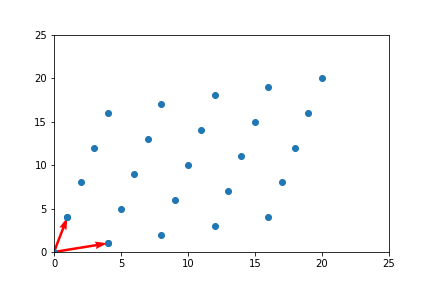
\includegraphics[scale=0.5]{lattice.png}
    \end{figure}
\end{frame}

%------------------------------------------------

\begin{frame}{Bullet Points}
    \begin{itemize}
        \item Lorem ipsum dolor sit amet, consectetur adipiscing elit
        \item Aliquam blandit faucibus nisi, sit amet dapibus enim tempus eu
        \item Nulla commodo, erat quis gravida posuere, elit lacus lobortis est, quis porttitor odio mauris at libero
        \item Nam cursus est eget velit posuere pellentesque
        \item Vestibulum faucibus velit a augue condimentum quis convallis nulla gravida
    \end{itemize}
\end{frame}


%------------------------------------------------

\begin{frame}{Blocks of Highlighted Text}
    In this slide, some important text will be \alert{highlighted} because it's important. Please, don't abuse it.

    \begin{block}{Block}
        Sample text
    \end{block}

    \begin{alertblock}{Alertblock}
        Sample text in red box
    \end{alertblock}

    \begin{examples}
        Sample text in green box. The title of the block is ``Examples".
    \end{examples}
\end{frame}

%------------------------------------------------

\begin{frame}{Multiple Columns}
    \begin{columns}[c] % The "c" option specifies centered vertical alignment while the "t" option is used for top vertical alignment

        \column{.45\textwidth} % Left column and width
        \textbf{Heading}
        \begin{enumerate}
            \item Statement
            \item Explanation
            \item Example
        \end{enumerate}

        \column{.5\textwidth} % Right column and width
        Lorem ipsum dolor sit amet, consectetur adipiscing elit. Integer lectus nisl, ultricies in feugiat rutrum, porttitor sit amet augue. Aliquam ut tortor mauris. Sed volutpat ante purus, quis accumsan dolor.

    \end{columns}
\end{frame}

%------------------------------------------------
\section{Second Section}
%------------------------------------------------

\begin{frame}{Table}
    \begin{table}
        \begin{tabular}{l l l}
            \toprule
            \textbf{Treatments} & \textbf{Response 1} & \textbf{Response 2} \\
            \midrule
            Treatment 1         & 0.0003262           & 0.562               \\
            Treatment 2         & 0.0015681           & 0.910               \\
            Treatment 3         & 0.0009271           & 0.296               \\
            \bottomrule
        \end{tabular}
        \caption{Table caption}
    \end{table}
\end{frame}

%------------------------------------------------

\begin{frame}{Theorem}
    \begin{theorem}[Mass--energy equivalence]
        $E = mc^2$
    \end{theorem}
\end{frame}

%------------------------------------------------

\begin{frame}{Figure}
    Uncomment the code on this slide to include your own image from the same directory as the template .TeX file.
    %\begin{figure}
    %\includegraphics[width=0.8\linewidth]{test}
    %\end{figure}
\end{frame}

%------------------------------------------------

\begin{frame}[fragile] % Need to use the fragile option when verbatim is used in the slide
    \frametitle{Citation}
    An example of the \verb|\cite| command to cite within the presentation:\\~

    This statement requires citation \cite{p1}.
\end{frame}

%------------------------------------------------

\begin{frame}{References}
    % Beamer does not support BibTeX so references must be inserted manually as below
    \footnotesize{
        \begin{thebibliography}{99}
            \bibitem[Smith, 2012]{p1} John Smith (2012)
            \newblock Title of the publication
            \newblock \emph{Journal Name} 12(3), 45 -- 678.
        \end{thebibliography}
    }
\end{frame}

%------------------------------------------------

\begin{frame}
    \Huge{\centerline{\textbf{The End}}}
\end{frame}

%----------------------------------------------------------------------------------------

\end{document}